%iffalse
\let\negmedspace\undefined
\let\negthickspace\undefined
\documentclass[journal,12pt,onecolumn]{IEEEtran}
\usepackage{cite}
\usepackage{amsmath,amssymb,amsfonts,amsthm}
\usepackage{algorithmic}
\usepackage{graphicx}
\usepackage{textcomp}
\usepackage{xcolor}
\usepackage{txfonts}
\usepackage{listings}
\usepackage{enumitem}
\usepackage{mathtools}
\usepackage{gensymb}
\usepackage{comment}
\usepackage[breaklinks=true]{hyperref}
\usepackage{tkz-euclide} 
\usepackage{listings}
\usepackage{gvv}                                        
%\def\inputGnumericTable{}                                 
\usepackage[latin1]{inputenc}     
\usepackage{xparse}
\usepackage{color}                                            
\usepackage{array}                                            
\usepackage{longtable}                                       
\usepackage{calc}                                             
\usepackage{multirow}
\usepackage{multicol}
\usepackage{hhline}                                           
\usepackage{ifthen}                                           
\usepackage{lscape}
\usepackage{tabularx}
\usepackage{array}
\usepackage{float}
\newtheorem{theorem}{Theorem}[section]
\newtheorem{problem}{Problem}
\newtheorem{proposition}{Proposition}[section]
\newtheorem{lemma}{Lemma}[section]
\newtheorem{corollary}[theorem]{Corollary}
\newtheorem{example}{Example}[section]
\newtheorem{definition}[problem]{Definition}
\newcommand{\BEQA}{\begin{eqnarray}}
\newcommand{\EEQA}{\end{eqnarray}}
\usepackage{float}
\usepackage{listings}
\usepackage{xcolor}
%\newcommand{\define}{\stackrel{\triangle}{=}}
\theoremstyle{remark}
\usepackage{ circuitikz }
%\newtheorem{rem}{Remark}
% Marks the beginning of the document
\begin{document}
\title{8.1.1}
\author{EE24BTECH11007 - Arnav Makarand Yadnopavit}
\maketitle
\renewcommand{\thefigure}{\theenumi}
\renewcommand{\thetable}{\theenumi}
\parindent 0px \textbf{Question:} Find the area of the region bounded by the curve $y^2=x$ and the lines $x=1$, $x=4$ and the x-axis in the first quadrant.\\
\solution\\
\textbf{Theoretical Solution:}\\
Finding Area
\begin{align}
    A&=\int^{b}_{a}y_2\brak{x}-y_1\brak{x}dx\\
    y_2\brak{x}&=\sqrt{x}\\
    y_1\brak{x}&=0\\
    b&=4\\
    a&=1\\
    A&=\int^{4}_{1}\sqrt{x}dx\\
    A&=\frac{2}{3}\sbrak{x^{\frac{3}{2}}}^4_1\\
    A&=\frac{2}{3}\sbrak{8-1}\\
    \therefore A&=4.66666666666667
\end{align}
\textbf{Computational Solution:}\\
Using the trapezoidal rule to get the area\\
The trapezoidal rule is as follows.
\begin{align}
    \int^{b}_{a} f\brak{x}dx\approx \sum^{N}_{k=1}\frac{f\brak{x_{k+1}}+f\brak{x_{k}}}{2}h
\end{align}
where
\begin{align}
    h=\frac{b-a}{N}
\end{align}
$\therefore$The difference equation obtained is\\
\begin{align}
    \int^{4}_{1} f\brak{x}dx=\sum^{N}_{k=1}\frac{\sqrt{x_{k+1}}+\sqrt{x_{k}}}{2}h\\
    h=0.00001\\
    N=300000
\end{align}
Using the code answer obtained is 4.66666666667341
\begin{figure}[h]
    \centering
    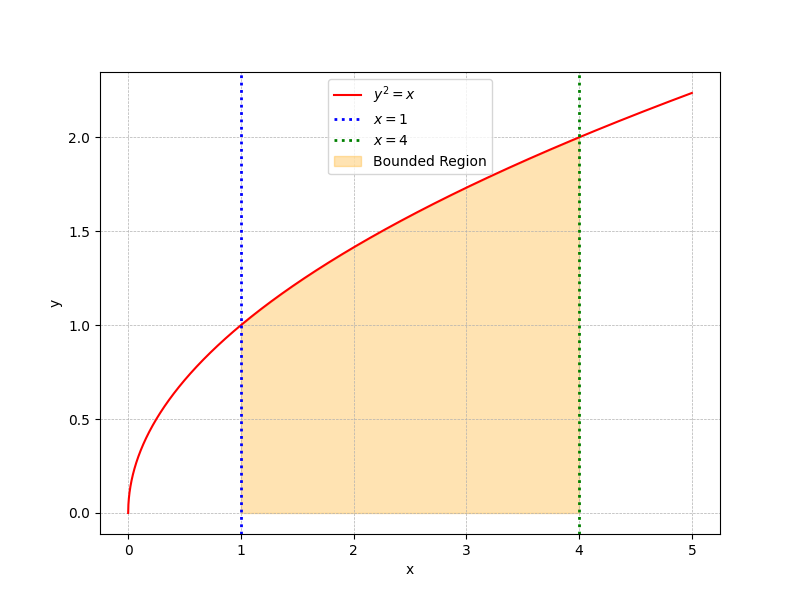
\includegraphics[width=\columnwidth]{figs/fig.png}
 \end{figure}
\end{document}

